\documentclass[11pt]{article}
\usepackage[T1]{fontenc}
\usepackage[utf8]{inputenc}%ATTENTION codage UTF8
\usepackage{fourier}
\usepackage[scaled=0.875]{helvet}
\renewcommand{\ttdefault}{lmtt}
\usepackage{amsmath,amssymb,makeidx}
\usepackage[normalem]{ulem}
\usepackage{diagbox}
\usepackage{fancybox}
\usepackage{tabularx}
\usepackage{colortbl}
\usepackage{xcolor}
\usepackage{tikz}
\usepackage{ulem}
\usepackage{pifont}
\usepackage{float}
\usepackage{multirow}
\usepackage{dcolumn}
\usepackage{enumitem}
\usepackage{textcomp} 
\usepackage{lscape}
%Sujet aimablement fourni par Marc Incamps
%Tapuscrit : Denis Vergès
\newcommand{\euro}{\eurologo{}}
\usepackage{graphics,graphicx}
\usepackage{pstricks,pst-plot,pst-tree,pstricks-add}
\usepackage{auto-pst-pdf}
\usepackage[left=3cm, right=3cm, top=2cm, bottom=2cm]{geometry}
\newcommand{\R}{\mathbb{R}}
\newcommand{\N}{\mathbb{N}}
\newcommand{\D}{\mathbb{D}}
\newcommand{\Z}{\mathbb{Z}}
\newcommand{\Q}{\mathbb{Q}}
\newcommand{\C}{\mathbb{C}} 
\renewcommand{\theenumi}{\textbf{\arabic{enumi}}}
\renewcommand{\labelenumi}{\textbf{\theenumi.}}
\renewcommand{\theenumii}{\textbf{\alph{enumii}}}
\renewcommand{\labelenumii}{\textbf{\theenumii.}}
\newcommand{\vect}[1]{\overrightarrow{\,\mathstrut#1\,}}
\def\Oij{$\left(\text{O}~;~\vect{\imath},~\vect{\jmath}\right)$}
\def\Oijk{$\left(\text{O}~;~\vect{\imath},~\vect{\jmath},~\vect{k}\right)$}
\def\Ouv{$\left(\text{O}~;~\vect{u},~\vect{v}\right)$}
\usepackage{fancyhdr}
\usepackage[french]{babel}
\usepackage{hyperref}

\usepackage[np]{numprint}
\begin{document}
\setlength\parindent{0mm} 
\setlength{\headheight}{13.59999pt} 
\pagestyle{fancy}
\thispagestyle{empty}
\begin{center}

{\Large \textbf{\decofourleft~Brevet blanc du 4 avril 2024~\decofourright}}

\bigskip

\textbf{Durée : 2 heures} 
\bigskip

\textbf{L'utilisation d'une calculatrice collège est autorisée.} 
\bigskip

\textbf{La notation tiendra compte du soin apporté à la rédaction et à la présentation.} \end{center}

\bigskip

\textbf{\large{}Exercice 1 \hfill 19 points}


\textbf{Question 1 :} Soit $f$, la fonction définie par $f(x) = -2x + 3$.

Quelle est la représentation de la fonction $f$ ? Justifiez la réponse.

\medskip

\begin{tabularx}{\linewidth}{*3{>{\centering\arraybackslash}X}}
\textbf{Réponse A}\rule[-7pt]{0pt}{0pt}
\psset{unit=0.4cm}
\def\xmin {-5}   \def\xmax {5} \def\ymin {-3}   \def\ymax {6}
\begin{pspicture*}(\xmin,\ymin)(\xmax,\ymax)
\psgrid[subgriddiv=1, gridcolor=lightgray]
\psaxes[arrowsize=3pt 2, ticksize=-2pt 2pt,Dx=2,Dy=2,labelFontSize=\scriptstyle]{->}(0,0)(\xmin,\ymin)(\xmax,\ymax) 
\psplot[linecolor=blue]{\xmin}{\xmax}{1.5 x mul 3 add}
\end{pspicture*}
&
\textbf{Réponse B}\rule[-7pt]{0pt}{0pt}
\psset{unit=0.4cm}
\def\xmin {-5}   \def\xmax {5} \def\ymin {-3}   \def\ymax {6}
\begin{pspicture*}(\xmin,\ymin)(\xmax,\ymax)
\psgrid[subgriddiv=1, gridcolor=lightgray]
\psaxes[arrowsize=3pt 2, ticksize=-2pt 2pt,Dx=2,Dy=2,labelFontSize=\scriptstyle]{->}(0,0)(\xmin,\ymin)(\xmax,\ymax) 
\psplot[linecolor=blue]{\xmin}{\xmax}{-2 x mul 3 add}
\end{pspicture*}
&
\textbf{Réponse C}\rule[-7pt]{0pt}{0pt}
\psset{unit=0.4cm}
\def\xmin {-5}   \def\xmax {5} \def\ymin {-3}   \def\ymax {6}
\begin{pspicture*}(\xmin,\ymin)(\xmax,\ymax)
\psgrid[subgriddiv=1, gridcolor=lightgray]
\psaxes[arrowsize=3pt 2, ticksize=-2pt 2pt,Dx=2,Dy=2,labelFontSize=\scriptstyle]{->}(0,0)(\xmin,\ymin)(\xmax,\ymax) 
\psplot[linecolor=blue]{\xmin}{\xmax}{3 x mul 2 sub}
\end{pspicture*}
\end{tabularx}

\medskip

\begin{minipage}{0.65\linewidth}\textbf{Question 2 :}
On considère la fonction $g$ dont la représentation graphique est donnée ci-contre.
\begin{itemize}
\item[(a)] Quelle est l'image de $2$ par $g$ ?
\item[(b)] Combien y a-t-il d'antécédents de $1$ par $g$ ? Citez-en un.
\end{itemize}

 
\end{minipage}\hfill
\begin{minipage}{0.28\linewidth}
\psset{unit=0.6cm}
\def\xmin {-3}   \def\xmax {3} \def\ymin {-3}   \def\ymax {3}
\begin{pspicture*}(\xmin,\ymin)(\xmax,\ymax)
\psgrid[subgriddiv=1, gridcolor=lightgray]
\psaxes[arrowsize=3pt 2, ticksize=-2pt 2pt,Dx=2,Dy=2,labelFontSize=\scriptstyle]{->}(0,0)(\xmin,\ymin)(\xmax,\ymax) 
\psplot[linecolor=blue]{\xmin}{\xmax}{-5 x dup mul mul 17 add x mul 6 div}
\psdots[linecolor=blue](-2,1)(-1,-2)(1,2)(2,-1)
\uput[dl](-2,1){\blue A} \uput[dl](-1,-2){\blue B} 
\uput[ur](1,2){\blue C} \uput[ur](2,-1){\blue D} 
\end{pspicture*}
\end{minipage}

\medskip

\textbf{Question 3 :}

On donne ci-dessous un tableau de valeurs de la fonction $h$ définie par $h(x) = - 2x + 3$ réalisé à l'aide d'un tableur :

\begin{center}
%\renewcommand{\arraystretch}{1.2}
$\begin{array}{|>{\cellcolor{lightgray}}c| *{8}{>{\centering\arraybackslash}m{1cm}|}}
\cline{2-9}
\rowcolor{lightgray} &\text A & \text B & \text C & \text D & \text E & \text F & \text G & \text H\\
\hline
1 & \blue $x$ & -3 & -2 & -1 & 0 & 1 & 2 & 3 \\ \hline
2 & \blue $h(x)$ & 9 & 7 & 5 & 3 & 1 & -1 & -3 \\ \hline
\end{array}$
\end{center}
\begin{itemize}
\item[(a)] Quelle formule a-t-on saisie dans la case B2 avant de l'étirer vers la droite ?
\item[(b)] Donnez l'image de $3$ par $h$. 
\item[(c)] Donnez un antécédent de $-1$ par $h$.

\end{itemize}



\medskip

\textbf{Question 4 :} On considère la fonction $k(x) = 2x - x(x-1)$. 
\begin{itemize}
\item[a.] Développez et réduisez l'expression de $k(x)$.
\item[b.] Calculez l'image de $\dfrac13$ en détaillant les étapes. 
\end{itemize}



\bigskip
 \newpage
 \textbf{\large{}Exercice 2 \emph{Dans cet exercice, toutes les questions sont indépendantes} \hfill 19 points}
 
 
\ \\


\begin{enumerate}
\item Factorisez l'expression $(x+3)(2x-4) + (x+3)(6x+1)$. 
\ \\
\item Sur la figure ci-dessous, qui n'est pas à l'échelle : \\$AC = 4,5$ cm, $CD = 1,5$ cm, $CE = 1$ cm et $BC = 3$ cm. \\
Les points $A$, $C$ et $D$ sont alignés. \\
Les points $B$, $C$ et $E$ sont alignés. \bigskip
\begin{figure}[H]
\begin{tikzpicture}
\draw (0,0) -- (4, 0.8) ; 
\draw (1, 0.2) -- (3.5, 3.7);
\draw (3, 0.6) -- (1.5, 3.3);
\draw (0,3) -- ( 4, 3.8) ; 
\draw (1, 0) node{$E$} (3, 0.4) node {$D$};
\draw (1.5, 3.55) node{$A$} (3.5, 3.9) node {$B$};
\draw (2, 2) node{$C$};
\draw (10, 2) node{
Démontrez que les droites $(AB)$ et $(ED)$ sont parallèles.};
\end{tikzpicture}
\end{figure}

\ \\

\item 
Un article coûte $34$ euros après avoir subi une réduction de $15$ \%. Quel était son prix avant réduction ? 

\ \\

\item Décomposez en produit de facteurs premiers le nombre $41\ 895$. Quel est le plus grand nombre premier divisant $41\ 895$ ? 


\ \\
\item Horatio, William, et Juliette ont respectivement $5$, $9$ et $11$ ans. Ils décident de partager $100$ chocolats en proportion de leurs âges, c'est-à-dire suivant le ratio $5:9:11$.\\ Donnez le nombre de chocolats reçu par chacun. 
\end{enumerate}

\newpage
 \textbf{\large{}Exercice 3   \hfill 18 points}
 

Lors d'une course en moto-cross, après avoir franchi une rampe, Gaëtan
a effectué un saut record en moto. Le saut commence dès que Gaëtan quitte la rampe. \\ On note $t$ la durée (en secondes) de ce saut. \\
La hauteur (en mètres) est déterminée en fonction de la durée $t$ par la fonction $h$ suivante\newline $h\colon t \mapsto (-5t -1,35)(t-3,7)$. \\
\begin{figure}[H]
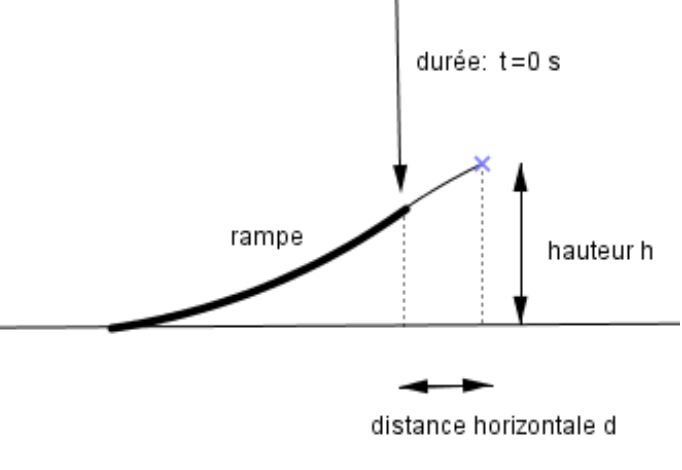
\includegraphics[scale=0.3]{Exo32.png}
\end{figure}
Voici la courbe représentative de cette fonction $h$. 
\begin{figure}[H]
\center
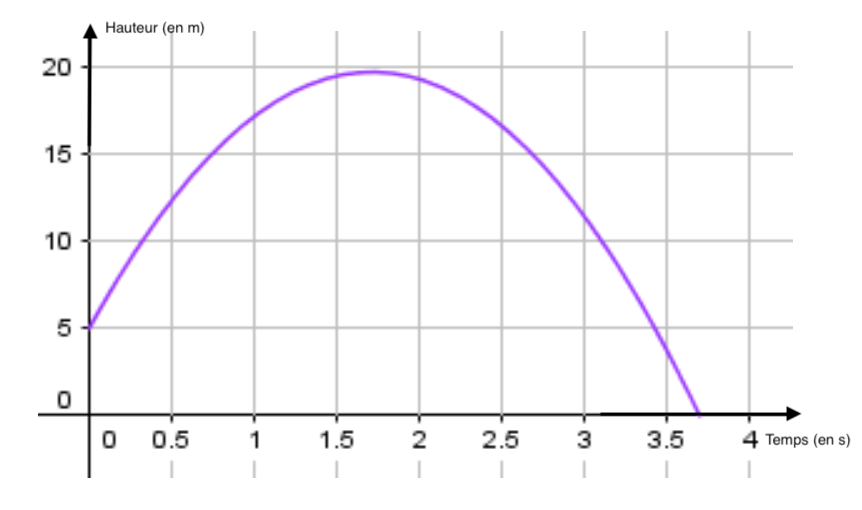
\includegraphics[scale=0.4]{Exo31.png}
\end{figure}
\begin{enumerate}
\item Développez et réduisez l'expression $h(t)$. 
\item \textbf{Par lecture graphique}, répondez aux questions suivantes : 
\begin{itemize}
\item[a.] Quelle est la hauteur maximale du saut ? Au bout de combien de temps est-elle atteinte ? 
\item[b.] Quelle est la durée du saut de Gaëtan ?
\item[c.] À quel(s) instant(s) Gaëtan est-il à $15$ m de haut ? 
\item[d.] Pendant combien de temps Gaëtan est-il à une hauteur supérieure à $10$ m ? 
\end{itemize}
\item \textbf{Calculez} $h(3,5)$ et interprétez le résultat. 
\item Au moment où Gaëtan quitte la rampe, montrez que sa hauteur est inférieure à $5$ mètres. 
\item À la fin de la course, à $17$ h $15$, Gaëtan rentre chez lui. Il habite à $7150$ m et a roulé en moto à une vitesse moyenne de $33$ kilomètres par heure. À quelle heure est-il arrivé chez lui ? 
\end{enumerate}

\newpage
 \textbf{\large{}Exercice 4   \hfill 12 points}
 
 On considère le programme de calcul suivant : \begin{itemize}
 \item[$\cdot$] Choisir un nombre. 
 \item [$\cdot$] Prendre le carré de ce nombre.
 \item [$\cdot$] Multiplier le résultat par $2$. 
 \item [$\cdot$] Ajouter le nombre de départ. 
 \item [$\cdot$] Soustraire $66$. 
 \end{itemize}
 \ \\
 \begin{enumerate}
 
 \item \begin{itemize}
 \item[a.] Montrez que si le nombre choisi au départ est $4$, le résultat obtenu est $-30$. 
 \item[b.] Quel résultat obtient-on si le nombre choisi au départ est $-3$ ? 
 \end{itemize}
 \ \\ 
 \item On s'intéresse au bloc d'instruction ci-dessous intitulé « Programme de calcul ». On souhaite le compléter pour calculer le résultat obtenu avec le programme de calcul en fonction du nombre choisi au départ. \\
 On précise que deux variables ont été créées : « nombre choisi » qui correspond au nombre choisi au départ, et « Résultat ». 
 \begin{figure}[H]
 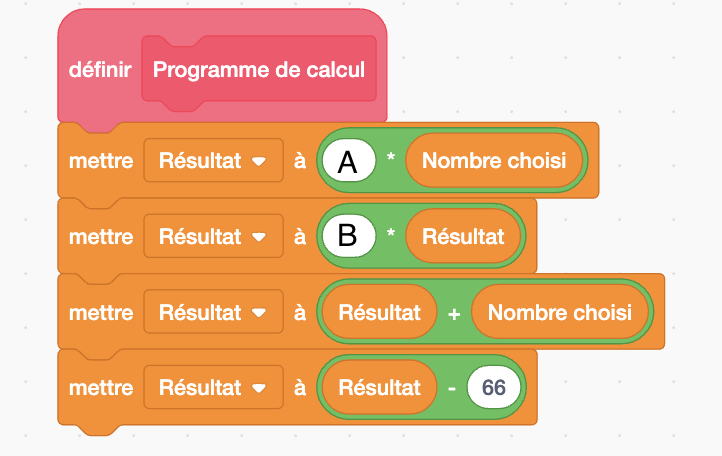
\includegraphics[scale=1]{Exo4}
 \end{figure}
 Écrivez sur votre copie le contenu qui doit être inséré dans les emplacements $A$ et $B$. \textbf{Aucune justification n'est attendue pour cette question.}
 
 \ \\ 
 \item On nomme $x$ le nombre de départ. \begin{itemize}
 \item[a.] Déterminez l'expression obtenue par le programme en fonction de $x$.
 \item[b.] Développez et réduisez $(2x-11)(x+6)$. Que peut-on en conclure ? 
 \end{itemize}
 \end{enumerate}
 
 
\newpage
 \textbf{\large{}Exercice 5   \hfill 16 points}
 
 
 Une famille se promène au bord d'une rivière. Les enfants aimeraient connaître la largeur de cette rivière. Ils prennent des repères, comptent leurs pas et dessinent le schéma ci-dessous sur lequel les points $C$, $E$ et $D$, de même que $A$, $E$ et $B$ sont alignés. (Le schéma n'est pas à l'échelle). 
 \begin{figure}[H]
 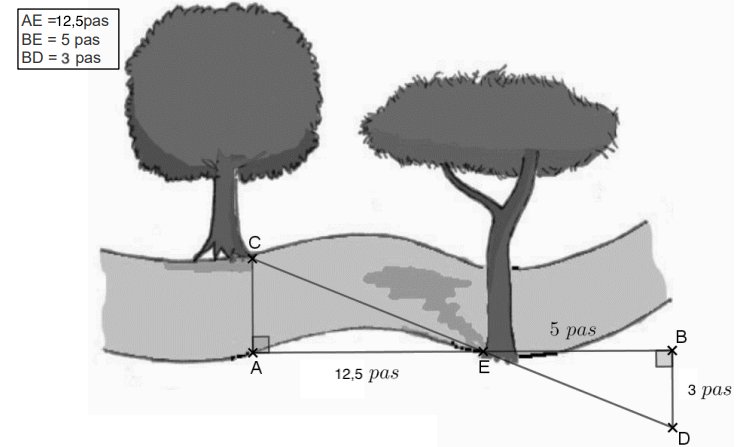
\includegraphics[scale=0.8]{riviere.png}
 \end{figure}
 
 \begin{enumerate}
 \item Démontrez que les droites $(AC)$ et $(BD)$ sont parallèles. 
 \item Déterminez en nombre de pas, la largeur $AC$ de la rivière. \\
 Pour les questions qui suivent, on assimile la longueur d'un pas à $65$ cm. 
 \item Montrez que la longueur $CE$ vaut $9,5$ m, en arrondissant au décimètre près. 
 \item \begin{itemize}
 \item[a.] L'un des enfants lâche un bâton dans la rivière au niveau du point $E$. Avec le courant, le bâton se déplace en ligne droite en $5$ secondes jusqu'au point $C$. \\ Calculez la vitesse du bâton en mètres par seconde. 
 \item[b.] Est-il vrai que « le bâton se déplace à une vitesse moyenne inférieure à $7$ km/h » ?
 \end{itemize}
 \end{enumerate}
 
 
\newpage
 \textbf{\large{}Exercice 6   \hfill 16 points}

\begin{enumerate}

\item Une abeille a une masse moyenne de $100$ mg et rapporte en moyenne 
$80$ mg de charge (nectar, pollen) à chaque voyage. 
Un homme a une masse de $75$ kg. S'il se chargeait proportionnellement à sa masse, comme une abeille, quelle masse cet homme transporterait-il ? 
\item Quand elles rentrent à la ruche, les abeilles déposent le nectar récolté dans des alvéoles. 

On considère que ces alvéoles ont la forme d'un prisme de $1,15$ cm de hauteur et dont la base est un hexagone d'aire $23$ mm${}^2$ environ, comme sur la figure ci-après. 


\begin{center}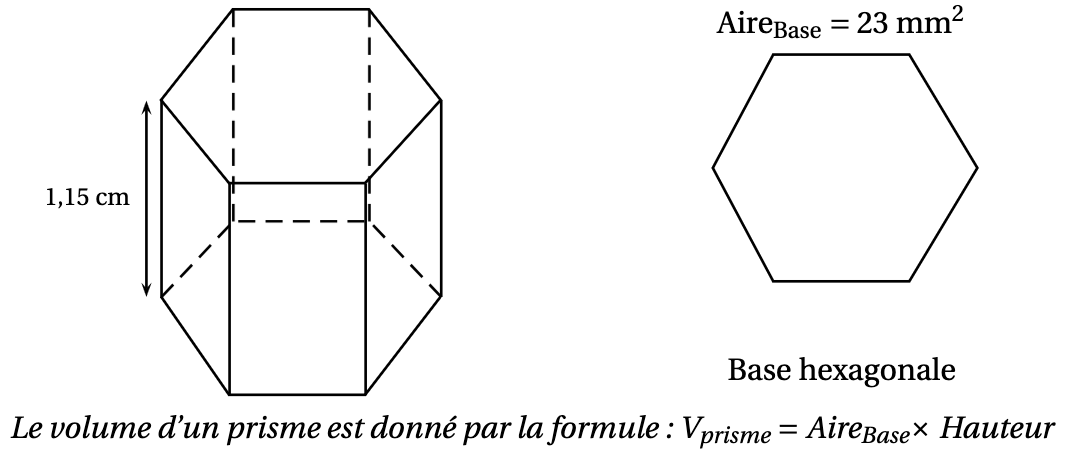
\includegraphics[width = 12 cm]{Exo61}
\end{center}
\begin{enumerate}
\item Vérifiez que le volume d'une alvéole de ruche est égal à $264,5$ mm${}^3$.

		\item L'abeille stocke le nectar dans son jabot. Le jabot est une petite poche sous l'abdomen d'un volume de $6 \times  10^{-5}$ litre. Combien de sorties au minimum l'abeille doit-elle faire pour remplir une alvéole ?

(rappel: 1 dm$^3$ = 1 litre) 
\end{enumerate}
\item Le graphique ci-dessous présente la production française de miel en 2015 et 2016.

\begin{center}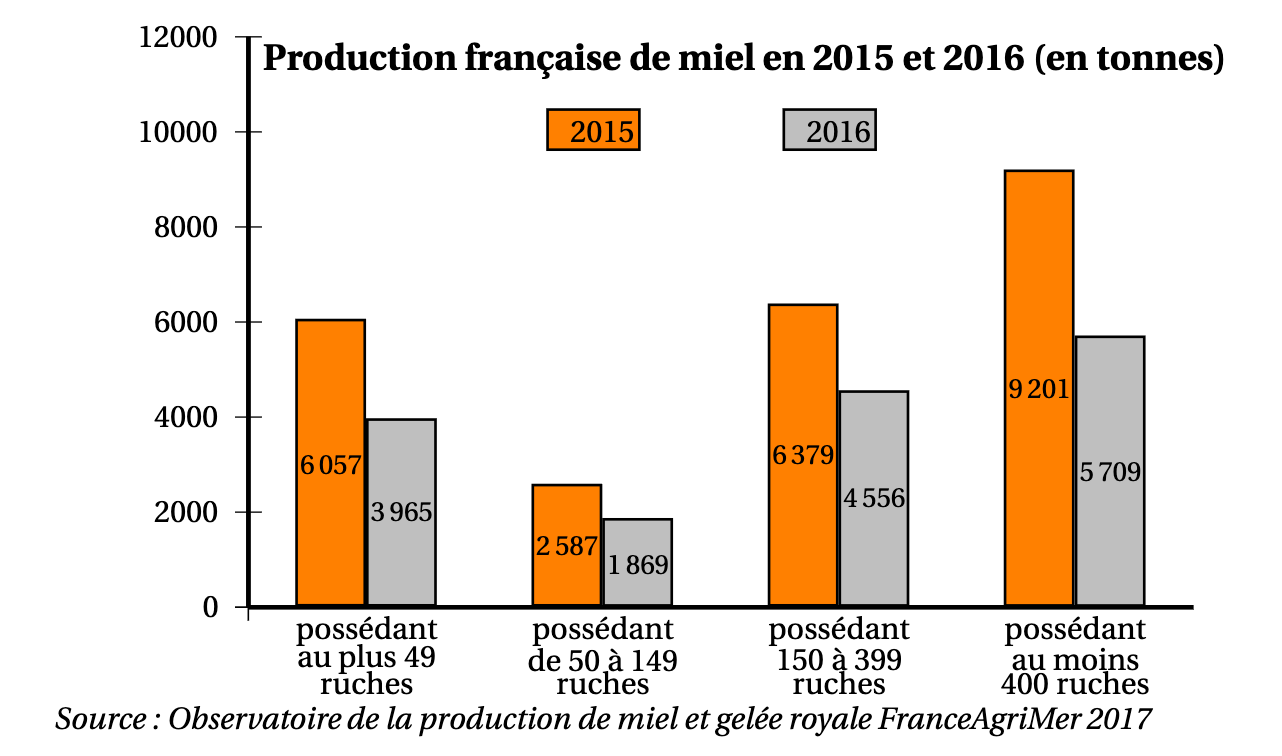
\includegraphics[width = 12 cm]{Exo62}
\end{center}

	\begin{enumerate}
		\item Calculer la quantité totale de miel (en tonnes) récoltée en 2016.
		\item Sachant que la quantité totale de miel récoltée en 2015 est de \np{24224} tonnes, calculer le pourcentage de baisse de la récolte de miel entre 2015 et 2016.
	\end{enumerate}
\end{enumerate}

\end{document}